\documentclass[tikz,border=10pt]{standalone}
\usetikzlibrary{shapes}
\usetikzlibrary{arrows}
\usetikzlibrary{positioning}
\begin{document} 
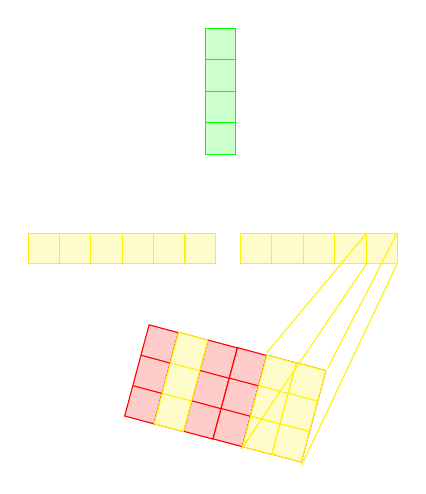
\begin{tikzpicture}[
  hid/.style 2 args={
    rectangle split,
    draw=#2,
    rectangle split parts=#1,
    fill=#2!20,
    outer sep=1mm},
  hidr/.style 2 args={
    rectangle split,
    rectangle split horizontal,
    draw=#2,
    rectangle split parts=#1,
    fill=#2!20,
    outer sep=1mm}
]

  \foreach \step in {1,...,6} {
    \node[hid={3}{red},rotate=-15,shift={(0,-.1 * \step)}] (e\step) at (.40*\step, -1) {};    
  }

  \foreach \step in {5,...,6} {
    \node[hid={3}{yellow},rotate=-15,shift={(0,-.1 * \step)}] (c\step) at (.40*\step, -1) {};    
  }
 
\node[hidr={5}{yellow}] (conv2) at (2.5,.5) {};

\draw[yellow] (1.84,-.82) -- (3.1,.69);
\draw[yellow] (1.51,-2.05) -- (3.105,.31);
\draw[yellow] (2.61,-1.02) -- (3.49,.69);
\draw[yellow] (2.28,-2.25) -- (3.495,.31);

  \foreach \step in {2,...,2} {
    \node[hid={3}{yellow},rotate=-15,shift={(0,-.1 * \step)}] (c\step) at (.40*\step, -1) {};    
  }
 
\node[hidr={6}{yellow}] (conv1) at (0,.5) {};

\node[hid={4}{green}] (s3) at (1.25, 2.5) {};
%\path[->] (concat) edge (s2);

\end{tikzpicture}

\end{document}
